\adparagraph{Adjusted nDCG}

\begin{figure}[H]
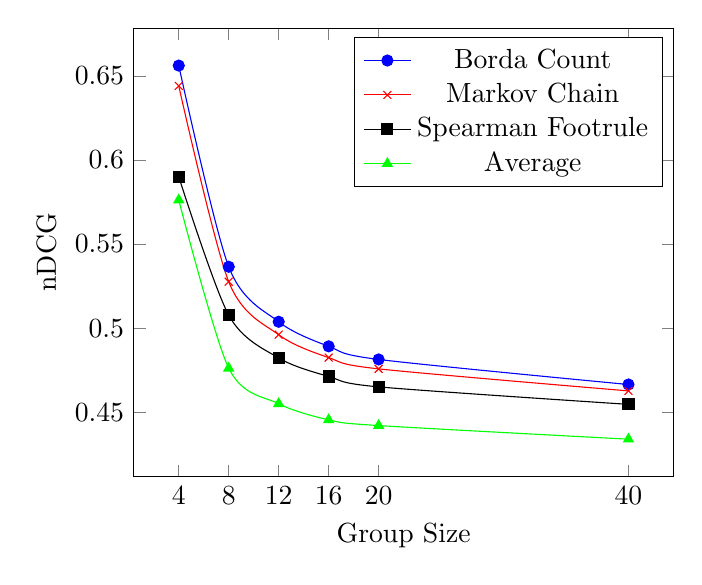
\begin{tikzpicture}
    \begin{axis}[
        xlabel=Group Size,
        ylabel=nDCG,
        xtick = {4,8,12,16,20,40}]
    \addplot[smooth,mark=*,blue] plot coordinates {
        (4,0.6561)
        (8,0.5365)
        (12,0.5038)
        (16,0.4892)
        (20,0.4814)
        (40,0.4665)
    };
    \addlegendentry{Borda Count}

    \addplot[smooth,color=red,mark=x] plot coordinates {
            (4,0.6440)
            (8,0.5276)
            (12,0.4961)
            (16,0.4825)
            (20,0.4758)
            (40,0.4627)
        };
    \addlegendentry{Markov Chain}
    
        \addplot[smooth,color=black,mark=square*] plot coordinates {
            (4,0.59)
            (8,0.5077)
            (12,0.4823)
            (16,0.4713)
            (20,0.4651)
            (40,0.4547)
        };
    \addlegendentry{Spearman Footrule}
    
    \addplot[smooth,color=green,mark=triangle*] plot coordinates {
            (4,0.5762)
            (8,0.4762)
            (12,0.4551)
            (16,0.4455)
            (20,0.4421)
            (40,0.434)
        };
    \addlegendentry{Average}
    
    \end{axis}
\end{tikzpicture}
\caption{Results for nDCG test}\label{fig:ndcg}
\end{figure}
